\subsubsection{Teorijska nastava}
\label{subsubsec:prijava za nastavu}
\begin{itemize}
  \item \textbf{Kratak opis}: Kandidat koji se upisao u auto školu počinje sa pohađanjem teorijske nastave u izabranoj grupi. 
  Predavač evidentira prisustvo kandidata na časovima teorije koje on drži.
  \item \textbf{Učesnici}:
    \begin{itemize}
    \item  Kandidat - korisnik sistema koji pohađa nastavu.
    \item  Predavač - korisnik koji drži časove i evidentira prisustvo.
    \end{itemize}
  \item \textbf{Preduslovi}:
    \begin{itemize}
    \item  Kandidat mora biti upisan u auto školu.
    \item  Kandidat mora biti raspoređen u grupu kod predavača.
    \item  Kandidat je izmirio  prethodne troškove upisa.
    \item  Predavač je zadužen za grupu koju kandidati pohađaju.
    \item  Predavač je ulogovan na sistem.
    \item  Sistem je u funkciji.
    \item  U sistemu ne postoji evidentiran čas za grupu u tekućem danu.
    \item  Predavač  ima pristup internetu.
    \end{itemize}
  \item \textbf{Postuslovi}:
      \begin{itemize}
      \item Kandidat je evidentiran da je pohađao nastavu.
      \item Predavač je evidentirao održano predavanje.
      \end{itemize}
  \item \textbf{Osnovni tok}:
      \begin{enumerate}
        \item Predavač otvara stranicu za evidenciju prisustva korisnika.
        \item Predavač popunjava formular za započinjanje časa sa grupom.
        \item Predavač potvrdjuje da zapocinje cas sa grupom.
        \item Sistem prikazuje listu kandidata koji pohađaju nastavu u toj grupi.
        \item Predavač evidentira prisustvo za svakog kandidata.
        \item Predavač zaključuje evidenciju.
        \item Predavač započinje predavanje.
        \item Predavač nakon održanog časa zaključuje čas.
        \item Sistem šalje mail svim učesnicima o uspešno završenom času i njihovom napretku. %ovo treba obrisati
      \end{enumerate}

  \item \textbf{Alternativni tokovi}:
      \begin{itemize}
        \item A1. \textbf{Neuspela validacija.}Ukoliku u koraku 2 sistem pronalazi neispravno polje formulara sistem obeležava polje koje treba ispraviti 
        crvenom bojom, a ispod polja piše  uzrok neispravnosti. Nakon ponovnog ispravnog unosa podataka proces se nastavlja u koraku 3 osnovnog toka.
      \end{itemize}
      
 \item \textbf{Specijalni zahtevi}:
      \begin{itemize}
        \item Polja formulara pri započinjanju časa su: grupa, termin, čas.
      \end{itemize}
\end{itemize}

\begin{figure}[H]
  \begin{center}
      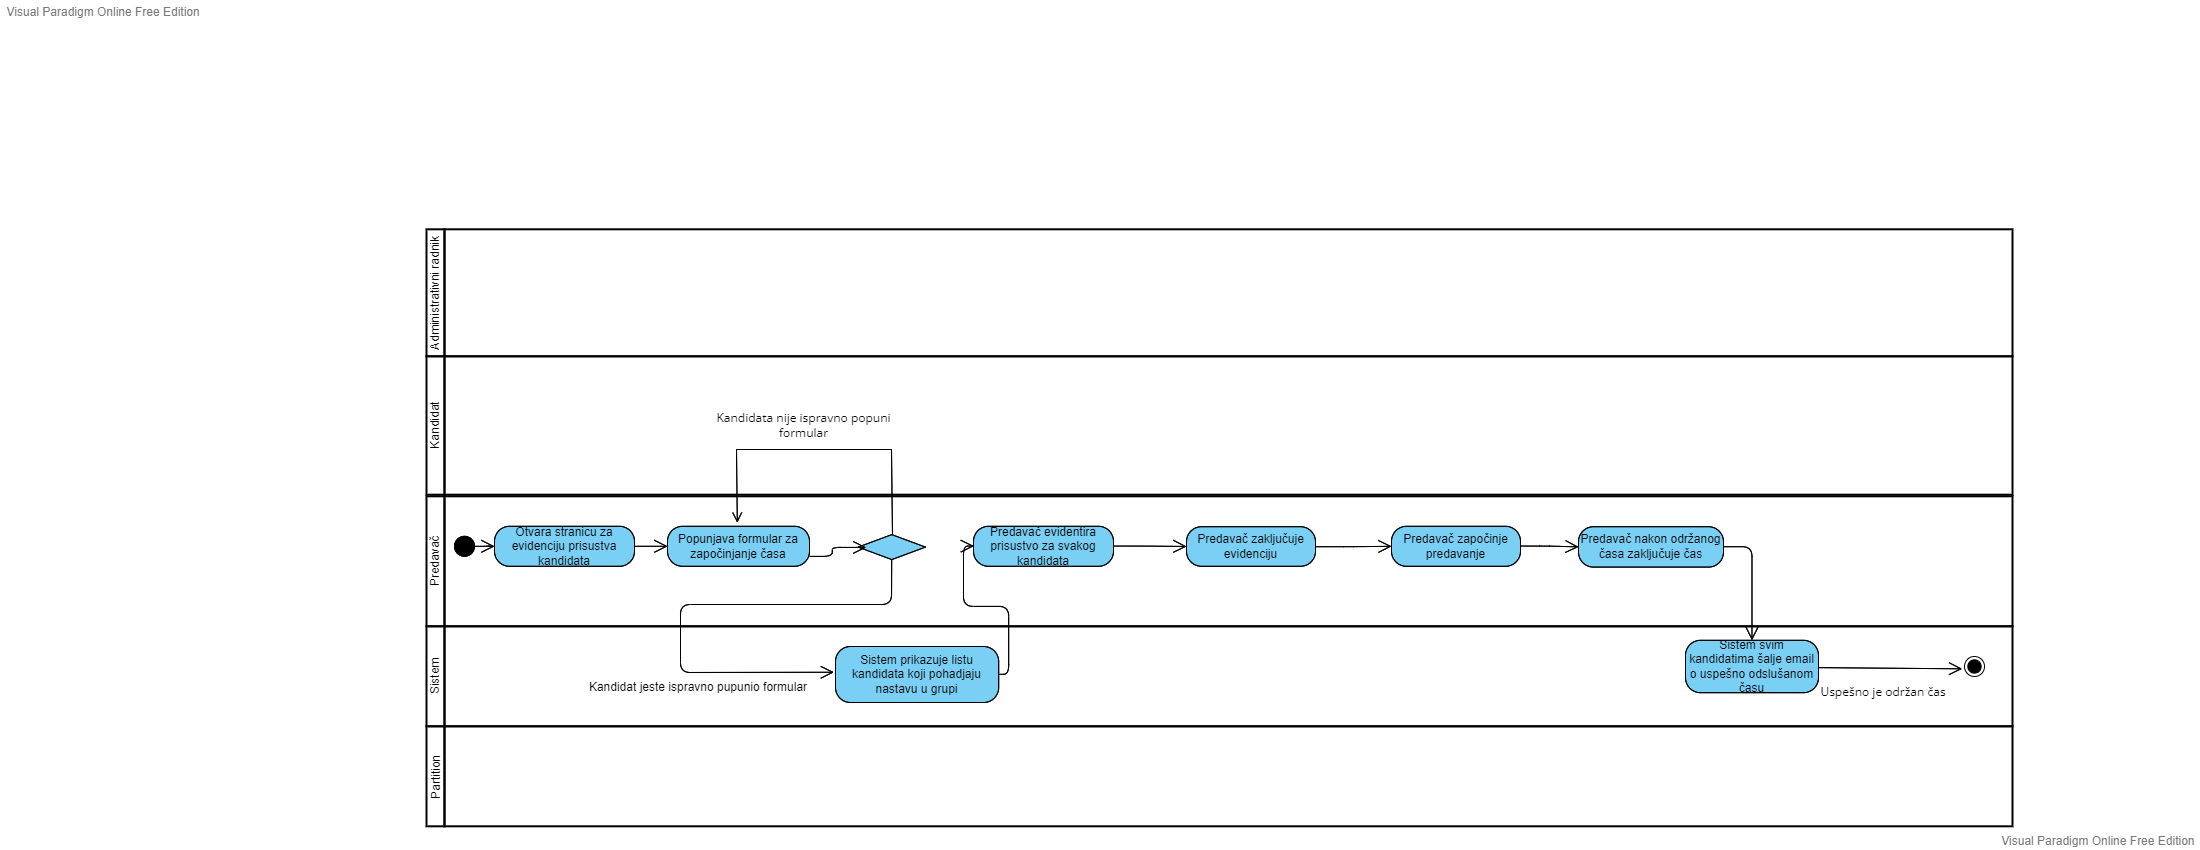
\includegraphics[width=140mm, height=70mm]{Diagrams/teorijska nastava dijagram.png}
  \end{center}
  \caption {Dijagram aktivnosti - teorijska nastava}
  \label{activity_diagram}

\end{figure}
